\documentclass[12pt]{article}
\def\activityid{F09-M-v2}\usepackage[letterpaper,margin=.65in,top=.60in,bottom=.65in]{geometry}
\usepackage[T1]{fontenc}
\usepackage[default]{sourcesanspro}
\usepackage{microtype,tikz,array,tabularx,fancyhdr,amsmath,amssymb}
\usepackage[hidelinks]{hyperref}
\usetikzlibrary{calc,arrows.meta}
\setlength{\parindent}{0pt}\setlength{\parskip}{7pt}
\setlength{\headheight}{0pt}\setlength{\footskip}{26pt}\setlength{\emergencystretch}{2em}
\pagestyle{fancy}\fancyhf{}\renewcommand{\headrulewidth}{0pt}\renewcommand{\footrulewidth}{.4pt}
\fancyfoot[L]{\scriptsize Bellingham Math Circle / Week 9 / \activityid}
\fancyfoot[R]{\scriptsize \thepage}
\definecolor{ink}{gray}{.12}\definecolor{soft}{gray}{.95}\color{ink}
\newcommand{\PageTitle}[2]{{\fontsize{10}{12}\selectfont\bfseries WEEK 9\quad BOUNCE LAB\hfill #1\par}\vspace{3pt}{\fontsize{26}{29}\selectfont\bfseries #2\par}\vspace{2pt}}
\newcommand{\NameLine}{{\small Name: \rule{2.65in}{.4pt}\hfill Date: \rule{1.35in}{.4pt}\par}\vspace{4pt}}
\newcommand{\Task}[2]{\par\vspace{3pt}{\large\bfseries #1}\par #2\par}
\newcommand{\Subhead}[1]{\par\vspace{3pt}{\large\bfseries #1}\par}
\newcommand{\RuleBox}[1]{\par\begingroup\setlength{\fboxsep}{8pt}\colorbox{soft}{\parbox{\dimexpr\linewidth-16pt\relax}{#1}}\endgroup\par}
\newcommand{\WriteBox}[2]{\par\textbf{#1}\par\vspace{2pt}\begin{tikzpicture}\draw[black!40,line width=.5pt] (0,0) rectangle (\dimexpr\linewidth-.5pt\relax,#2);\end{tikzpicture}\par}
\newcommand{\StudentFooter}{\vfill{\small Try it with objects. Explain by pointing, talking, or drawing.}\par}
\newcommand{\RookBoard}[3]{\begin{tikzpicture}[x=#3,y=#3]\draw[step=1,black!45] (0,0) grid (#1,#2);\draw[thick] (0,0) rectangle (#1,#2);\node[font=\Large] at ({#1-.5},.5){$\star$};\draw[-{Latex},thick] (0,-.35)--(#1,-.35);\draw[-{Latex},thick] ({#1+.35},#2)--({#1+.35},0);\end{tikzpicture}}
\newcommand{\Table}[3]{\begin{tikzpicture}[x=#3,y=#3]\draw[step=1,black!25] (0,0) grid (#1,#2);\draw[thick] (0,0) rectangle (#1,#2);\fill (0,0)circle(3pt);\draw[-{Latex},very thick] (0,0)--(.7,.7);\node[below] at ({#1/2},-.1){width #1};\node[rotate=90,above] at (-.2,{#2/2}){height #2};\end{tikzpicture}}
\newcommand{\GraphNodes}{\coordinate(A)at(0,0);\coordinate(B)at(3,0);\coordinate(C)at(1.5,2.6);\coordinate(D)at(1.5,.95);}
\newcommand{\Kfour}[1]{\begin{tikzpicture}[scale=#1]\GraphNodes\draw[very thick](A)--(B)--(C)--(A)--(D)--(B) (D)--(C);\foreach \n in {A,B,C,D}{\node[circle,draw,fill=white,minimum size=22pt,font=\bfseries]at(\n){\n};}\end{tikzpicture}}
\newcommand{\House}[1]{\begin{tikzpicture}[scale=#1]\coordinate(A)at(0,0);\coordinate(B)at(3,0);\coordinate(C)at(3,2);\coordinate(D)at(0,2);\coordinate(E)at(1.5,3.3);\draw[very thick](A)--(B)--(C)--(D)--(A) (D)--(E)--(C);\foreach \n in {A,B,C,D,E}{\node[circle,draw,fill=white,minimum size=22pt,font=\bfseries]at(\n){\n};}\end{tikzpicture}}

\begin{document}

\PageTitle{GRADES 2--3}{Unbounce the ball}\NameLine
\RuleBox{Start at the bottom-left dot, at a 45-degree angle. At a side wall reverse left/right; at a top or bottom wall reverse up/down. Stop at the FIRST corner.}
\Task{1. Find a route.}{Trace this table. Mark each bounce and the final corner.}
\begin{center}\Table{2}{3}{.62in}\end{center}
\Task{2. Instead of bouncing, copy the room.}{Below are mirror copies of that table. Continue the path as one straight diagonal. Mark the \emph{first} point where it meets both a thick vertical and a thick horizontal wall.}
\begin{center}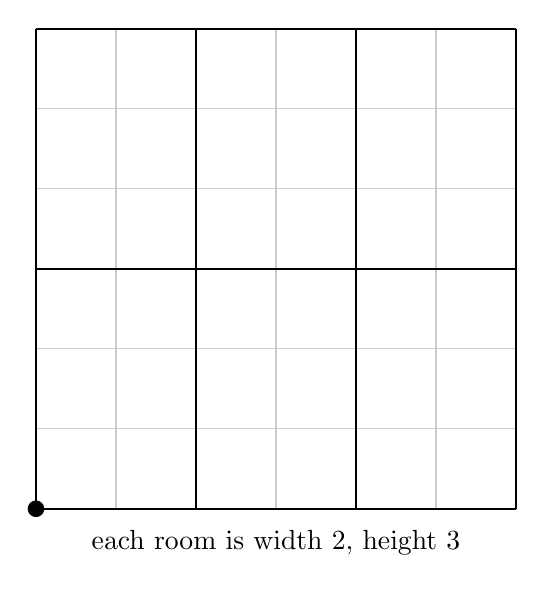
\begin{tikzpicture}[x=.40in,y=.40in]\draw[step=1,black!20](0,0)grid(6,6);\foreach\x in{0,2,4,6}{\draw[thick](\x,0)--(\x,6);}\foreach\y in{0,3,6}{\draw[thick](0,\y)--(6,\y);}\fill(0,0)circle(3pt);\node[below]at(3,-.15){each room is width 2, height 3};\end{tikzpicture}\end{center}
\textbf{Explain with a fold or your hands:} Why does crossing into a mirror room stand for a bounce in the original room?
\StudentFooter

\newpage

\PageTitle{GRADES 2--3}{When do two walls meet?}\NameLine
\Task{3. Count in two rhythms.}{For a width-2, height-3 table, thick vertical walls occur after 2, 4, 6, \ldots\ horizontal units. Thick horizontal walls occur after 3, 6, 9, \ldots\ vertical units. On a 45-degree path, those distances are equal.}
What is their first shared distance? Why would an earlier number fail?
\Task{4. Predict before drawing.}{Use copied rooms, lists of multiples, or a sketch. Count the number of room widths and heights to that first meeting.}
\begin{center}\renewcommand{\arraystretch}{1.9}\begin{tabular}{c|c|c|c|c}Width&Height&First shared&Widths&Heights\\\hline2&3&&&\\3&6&&&\\3&9&&&\\4&6&&&\end{tabular}\end{center}
\textbf{Fold back mentally:} Crossing one whole room width takes you to the right, two to the left, three to the right. What do room heights tell you? Predict the ending corner in each row.
\WriteBox{A prediction and a reason:}{.85in}
\Task{5. Design a challenge.}{Make a rectangle that ends at the top-right \emph{after at least one bounce}. Then make a table ending at the top-left. Give your partner the sizes and keep your explanation hidden.}
\WriteBox{My two sizes, corners, and checks:}{.85in}
\StudentFooter

\end{document}
